\documentclass[a4paper,titlepage]{scrartcl}
\pagestyle{plain}
\usepackage[utf8]{inputenc}
\usepackage[T1]{fontenc}
\usepackage[german]{babel}
\usepackage{float}
\usepackage{graphicx}
\usepackage{amsmath,amssymb,amstext}
\usepackage{enumerate}
\usepackage{units}

\numberwithin{equation}{section}

\title{Versuch P2-53: Franck-Hertz-Versuch\\Vorbereitung}
\author{Gruppe Di-22\\Genti Saliu, Jonas Müller}
\date{09. Mai 2014}

\begin{document}
	\begin{titlepage}
		\maketitle
		\thispagestyle{empty}
	\end{titlepage}
	
\newpage
\pagenumbering{roman}
\tableofcontents

\newpage
\pagenumbering{arabic}

\section{Einführende Versuche}
In diesem Praktikum wird der Franck-Hertz-Versuch durchgeführt. Mit diesem Versuch lässt sich zeigen, dass Atome nur diskrete Energiezustände annehmen können, und nicht wie in der klassischen Physik angenommen, jedes beliebige Energieniveau.

\subsection{Schaltung des Franck-Hertz-Versuchs}

Folgendes Schaltbild zeigt einen vereinfachten Aufbau einer Franck-Hertz-Röhre:

\begin{figure}[H]
	\centering
	\begin{tabular}{@{}r@{}}
		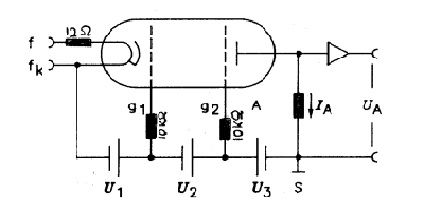
\includegraphics[width=0.4\textwidth]{bilder/schaltplan.jpg}\\
		\footnotesize\sffamily\textbf{Quelle:} Vorbereitungshilfe \cite{vorbereitungshilfe}
	\end{tabular}
	\caption{Schaltplan der Franck-Hertz-Röhre}
\end{figure}

Die Röhre an sich ist mit Quecksilbergas gefüllt. Auf der linken Seite befindet sich eine Glühwendel, die als Kathode fungiert. Über die Anschlüsse $f$ und $f_k$ wird Glühwendel mit Strom versorgt und erhitzt, es werden Elektronen emittiert.\\
$g_1$ ist ein grobmaschiges Anodengitter, welches positiv gegen die Glühwendel geladen ist. Die an $g_1$ angelegte Spannung $U_1$ beschleunigt die Elektronen in Richtung von $g_2$, welche dann mit den Hg-Atomen zusammenstoßen. Durch die positive Ladung des Gitters werden die Elektronen bewegen sich diese langsam zum Gitter hin. Elektronen, die durch das Gitter durch wandern, können dann dahinter beschleunigt werden, über die Spannung lässt sich dadurch die Anzahl dieser variieren. Würde man eine zu geringe (oder keine) Spannung anlegen, so würden sich die Elektronen langsam gleichmäßig im Raum verteilen (bis sie in die Nähe der Anode $g_2$ kommen). Außerdem erfahren die emittierten Elektronen noch eine geringe Beschleunigung in Richtung $g_1$, dieser Effekt wird aber erst in Aufgabe 1.4 wichtig.\\
$g_2$ ist eine feinmaschiges Anodengitter, an dem eine Beschleunigungsspannung $U_2$ anliegt. Durch die Potentialdifferenz zwischen $g_1$ und $g_2$ werden die Elektronen in Richtung $g_2$ beschleunigt. Im Bereich zwischen den Gittern kommt es dann auch zu elastischen sowie unelastischen Stößen zwischen den Elektronen und den Hg-Atomen.\\
Am rechten Ende Röhre befindet sich schließlich noch ein Auffangschirm A. Um diesen zu erreichen müssen die Elektronen noch die Bremsspannung $U_3$ überwinden. Sobald die Elektronen auf A auftreffen, kommt es zu einer Potentialdifferz $U_A$. Diese ist allerdings so gering, dass ein Verstärker benötigt wird um sie zu messen.\\
Elektronen, die durch die in der Röhre beschleunigt wurden, stoßen zunächst (bei geringer Beschleunigungsspannung) nur elastisch mit den Hg-Atomen zusammen. Der Grund dafür ist, dass die Elektronen zu wenig kinetische Energie (durch die Beschleunigung) besitzen, als das sie die Atome anregen können. Bei diesen elastischen Stöße wird kaum Energie übertragen, was dazu führt, dass die Elektronen das Gegenfeld vor dem Auffangschirm überwinden können. D.h. erhöht man die Beschleunigungsspannung, so erhöht sich auch $I_A$ welcher zwischen der Masse (S) und Auffangschirm fließt. Erreicht ein Elektronen allerdings eine Energie von $\unit[4,89]{eV}$, was der geringsten Anregungsenergie der Hg-Atome entspricht, so kann es seine gesamte bzw. einen Großteil seiner Energie durch einen unelastischen Stoß abgeben. Dabei wird dsd Hg-Atom auf ein höheres Energieniveau gehoben und die kinetische Energie des Elektron wird verringert, dass es den Auffangschirm nicht mehr erreichen kann. Dies hat zur Folge, dass die Spannung $U_A$ sinkt. Je mehr Elektronen Energie bei den Stößen abgeben haben, desto niedriger sinkt $U_A$ (hier sei schon angemerkt, dass nicht alle Elektronen zwingend Stoßen müssen, siehe 1.4). Erhöht man die Beschleunigungsspannung weiter, so steigt auch $U_A$ wieder, da die Elektronen genug Energie für den Stoß und das Gegenfeld haben. Erreichen die Elektronen eine kinetische Energie, welche groß genug für zwei Stoße ist, so sinkt $U_A$ wieder. Der gesamte Vorgang wiederholt sich mehrere Male.\\
Trägt man die gemessene Spannung $U_A$ (bzw. den Strom $I_A$) über die Beschleunigungsspannung $U_2$ auf, so ergibt sich eine typische Franck-Hertz-Kurve:

\begin{figure}[H]
	\centering
	\begin{tabular}{@{}r@{}}
		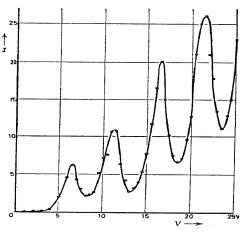
\includegraphics[width=0.4\textwidth]{bilder/franck_hertz_kurve.jpg}\\
		\footnotesize\sffamily\textbf{Quelle:} Vorbereitungshilfe \cite{vorbereitungshilfe}
	\end{tabular}
    \label{fig:aufgabe11}
	\caption{Franck-Hertz-Kurve}
\end{figure}

\subsection{Energie der niedrigsten Anregung von Quecksilber, Kontaktspannung zwischen Kathode und Anode}
Es soll in diesem Versuch die Energie der niedrigsten Anregung von Quecksilber bestimmt werden, d.h. die Energie, die ein Elektron besitzen muss, um ein Quecksilberatom aus dem Grundzustand in ein angeregtes Zustand zu bringen.\\ \\
Ausserdem soll die Kontaktspannung bestimmt werden, also diejenige Spannung, die aufgrund der verschiedenen Materialien von Kathode und Anode entsteht, die der Beschleunigungsspannung von Elektronen überlagert ist.\\ \\
Man muss dazu folgendermaßen vorgehen:
\begin{itemize}
\item Kathodenheizung einschalten
\item Quecksilberröhre mit der Offenheizung schrittweise $\unit[170]{^{\circ}C}$ (Schritte: $\unit[120]{^{\circ}C}$, $\unit[140]{^{\circ}C}$, $\unit[150]{^{\circ}C}$, $\unit[160]{^{\circ}C}$, $\unit[170]{^{\circ}C}$) aufheizen. \textbf{Röhre nie über $\unit[190]{^{\circ} C}$ erhitzen.} Mit der Temperatur steuert man die Anzahl der Hg-Atome, da die Röhre flüssiges Quecksilber enthält, das mit steigender Temperatur verdampft.\\ \\ Damit steigt auch die mittlere freie Weglänge $\lambda$:
\begin{equation}
\lambda=\frac{kT}{p \sigma}
\end{equation}
wobei $k=\unit[1.38 \cdot 10^{-23}]{\frac{J}{K}}$ die Boltzman-Konstante, $T$ die Temperatur der Röhre, $p$ der Druck und $\sigma\approx \unit[8 \cdot 10^{-6}]{cm^2} $ die Querschnittsfläche der Hg-Atome. Der Druck hängt von der Temperatur ab und für Quecksilber im Temperaturbereich $\unit[0]{^{\circ}C}$ bis $\unit[250]{^{\circ}C}$ gilt ungefähr:
\begin{equation}
p=\unit[8.7 \cdot 10^7]{mbar} \cdot 10^{\frac{-3110}{T}}
\end{equation}
\item Spannung am Raumladungsgitter $U_1$ einstellen, so dass genügend Elektronen ins Beschleunigungsfeld gelangen können.
\item Gegenspannung $U_3$ einstellen, so dass möglichst wenige Elektronen den Auffangschirm erreichen.
\end{itemize}
Für jeden Temperaturschritt sollte die optimale Franck-Hertz-Kurve ($I_A$ über $U$) mit Oszilloskop aufgenommen werden. Aus den aufgezeichneten Daten kann die Energe für die niedrigste beobachtbare Anregung von Quecksilber durch Elektronenstoß. Aus den Strommaxima (s. Bild \ref{fig:aufgabe11}) sind gleichmäßige Abstände $\Delta U$ zu erkennen.

\subsection{Messung des Anodenstroms}

In diesem Versuch soll bei einer Temperatur von $t \approx \unit[100]{^\circ C}$ der Zusammenhang zwischen Beschleunigungsspannung und Anodenstrom $I_{g_2}$ gemessen werden. Es gilt eine modifizierte Version des Raumladungsgesetzes:

\begin{equation*}
I_{g_2} \approx \lambda U^{\frac{3}{2}}
\end{equation*}

Durch geschicktes Auftragen soll die $U^{\frac{3}{2}}$-Abhängigkeit deutlich gemacht werden, dazu formt man die Gleichung um (logarithmieren) und trägt $I_{g_2}$ über die Beschleunigungsspannung U auf (bzw. deren Logarithmen):

\begin{equation*}
\ln{I_{g_2}} =  \frac{3}{2} \cdot \left( \log{\lambda} + \ln{U} \right)
\end{equation*}

Die Anodenspannung zeigt dabei keinen Franck-Hertz-Kurve, da ja alle Elektronen, besonders solche mit geringer kinetischer Energie, am Anodengitter ankommen, denn es gibt kein Gegenfeld zu überwinden.

\subsection{Bestimmung der Ionisierungsarbeit von Quecksilber}
Ionisierung durch Elektronenstoß tritt ab einer Elektronenenergie von $\unit[10.44]{eV}$ auf. Dabei verlassen Elektronen das Atom. Die Ionisierung macht sich dadurch bemerkbar, dass im Gasraum positive Ionen, die die Raumladung in Kathodennähe herabsetzen und im Anoden-Auffänger-Raum auftreten, die einen Strom umgekehrtes Vorzeichens gegenüber den Elektronenstrom bewirken.

\begin{description}
\item[Messung des Anodenstroms in Abhängigkeit von Anodenspannung] Die positiven Ione werden von der Glühkathode angezogen und aufgrund der dort höheren negativen Raumladung können sich mit Elektronen rekombinieren (dabei werden Photonen emittiert). Dadurch wird die Raumladung verringert und die Kathode emittiert mehr Eleketronen. Dadurch wird ab Ionisierungsenergieschwelle ein sehr steiler Anstieg des Anodenstroms.
\item[Plotten des Auffängerstroms] Die positiven Ionen treten auch auf dem Anoden-Auffänger-Raum und bewirken dort einen Strom umgehrtes Vorzeichens gegenüber des Auffängerstroms, d.h. ab Ionisation wird der Auffängerstrom $I_A$ kleiner.
\end{description}

\newpage
\subsection{Beobachtung der Emissionslinien bei brennender Gasentladung}

Bei der Rekombination der Ionen (Wiederaufnahme von Elektronen) kommt es zur Photonenemission. Mit einem Taschenspektrometer soll das dabei erzeugte Spektrum beobachtet werden. Laut $\cite{vorbereitungshilfe}$ sollte die hervortretenden Spektrallinien violett ($\unit[405]{nm}$, $\unit[408]{nm}$, $\unit[436]{nm}$), blau ($\unit[493]{nm}$), grün ($\unit[546]{nm}$) und gelb ($\unit[597]{nm}$) sein. Ohne Spektrometer ist eine fahles blaues Licht zu erkennen, was eine Überlagerung der Wellenlängen darstellt.\\
Da hier nur sehr kleine Ströme fließen, kann der Spannungsabfall am Widerstand i.A. vernachlässigt werden.

\newpage
\section{Bestimmung der nächst höheren Anregungsenergie}

Wie in Aufgabe 1.4 soll hier die Stoßwahrscheinlichkeit verringert werden, dabei wird also wieder das Raumladungsgitter $g_1$ als Beschleunigungsgitter verwendet. Da allerdings nur die nächst höhere Anregungsenergie erreichen wollen und keine Gasentladung wie zuvor, muss darauf geachtet werden, dass die Beschleunigungsspannung nicht zu hoch eingestellt wird.\\
Nun muss man wiederum die Einstellungen am Oszilloskop optimiert werden um eine Franck-Hertz-Kurve aufzunehmen, aus der man dann auf die zweitniedrigste Anregungsenergie schließen kann. Die entstehende Franck-Hertz-Kurve ist in erster Linie eine Linearkombination der ersten beiden Anregungsstufen, da die niedrigste Anregungsstufe nicht unterdrückt werden kann. Höhere Anregungsstufen werden, wenn dann nur sehr schwach angedeutet.

\section{Bestimmung der mittleren Energie der hauptsächlichen Anregung von Neon}

In diesem Versuch wird nun eine Neon-Röhre genutzt deren Schaltplan analog zum dem der Quecksilber-Röhre ist. Der Aufbau ist schon vollständig vorhanden. Es wird wiederum eine Franck-Hertz-Kurve aufgenommen, aus der die mittlere Anregungsenergie von Neon bestimmt werden soll. Man spricht hier von einer mittleren Energie, da es sich bei Neon um eine Gruppe von Energieniveaus handelt, die innerhalb eines Intervalls von ca. $\unit[0,5]{eV}$ breite liegen.\\
Neon ist bei Raumtemperatur bereits gasförmig, außerdem gilt das sich Neon annähernd wie ein ideales Gas verhält und deshalb $pV = nk_B T$. Der Druck ist also proportional zur Temperatur, weshalb eine Erhöhung der Temperatur keinen Einfluss auf die mittlere freie Weglänge hat:

\begin{equation*}
\lambda = \frac{k_b \cdot T}{p \cdot \sigma}
\end{equation*}

 Es könnte sich höchstens die thermische Bewegung der Teilchen verändern, so dass es im Mittel zu mehr Stößen kommt. Insgesamt ist es aber eher unnötig die Röhre zu heizen.
 
\newpage
\bibliographystyle{plain}
\bibliography{quellen}

\end{document}